\documentclass[11pt, a4paper]{article}
\usepackage{graphicx}
\usepackage{fullpage}
\begin{document}

\title{Physkalisches Praktikum\\Versuch M1\\08.11.18}
\author{Janosch Ehlers, Lenard Ansmann, Gruppe C8}
\maketitle

\textbf{Abstract}\\In diesem Versuch soll anhand der Schwingungsdauer eines Fadenpendels in Relation zur Änderung seiner Länge die Erdbeschleunigung g experimentell bestimmt werden.
\\

\textbf{Theoretischer Hintergrund}\\Ein Fadenpendel ist eine Kugel mit der Masse m, welche mittels eines Fadens an einem festen Punkt befestigt werden kann. Diese genannte Masse macht dabei den Großteil der Gesamtmasse aus, ihr Mittelpunkt stellt dabei näherungsweise den Schwerpunkt des Systems dar. Durch die Schwerkraft wird das Pendel automatisch in den Zustand des geringsten Potenziellen Energie gebracht. D. h. das Pendel wird in die Position mit dem geringsten Abstand zum Massenmittelpunkt der Erde ausgelenkt. Für gewöhnlich ist diese Position auf einer Linie mit dem Fixierpunkt und scheinbar identisch mit der lokalen Orthogonalen zum Boden. Diese Position wird im Folgenden als Ruhepunkt /-Position bezeichnet. Bringt man nun die Masse aus der Ruheposition, wird das Energie Potenzial erhöht. Da $E_{Pot} = m\cdot g\cdot h$ ist und h , welches hier die Höhe darstellt, sich vergrößert hat, hat sich die potenzielle Energie nun auch erhöht. Da es einen energetisch niedrigeren Zustand gibt, wird nun das Pendel von der Gravitation Richtung Massenmittelpunkt der Erde beschleunigt. Diese Beschleunigung entspricht nicht der Richtung des Fadens, kann aber in Teil Kräfte zerlegt werden. So gilt: $$F = m\cdot g$$ und da sich die Kugel auf einem Teilstück eines Kreisbogens mit der Auslenkung $\varphi$ bewegt: $$F=-m\cdot g\cdot Sin(\varphi)$$ Bezieht man nun mit ein, dass die Kugel für das Bogenstück $\Delta x = L \Delta \varphi$ die Zeit $\Delta t$ benötigt und  sich mit der Geschwindigkeit $v = \Delta x/ \Delta t$ bewegt, lässt sich nach der Zeit t abgeleitet folgende Relation bestimmen: $$ F= m\cdot L\cdot \varphi $$ Das Pendel benötigt eine Periodendauer von $2\pi$: $$ T=2\pi\cdot\sqrt{L\cdot g}$$ Da die Pendellänge nur schwer exakt bestimmbar ist, eine Längenänderung des Fadens aber schon, kann $L+L_i$ eingesetzt und nach g aufgelöst werden, um die Abhängigkeit der Pendellänge gegen die Periodendauer in Sekunden aufzutragen.$$m=\frac{T_{2i}-T_{2j}}{L_i-L_j}=\frac{4\pi^2}{g}$$ also ist: $$g=\frac{4\pi^2}{m}$$ 

\textbf{Aufbau und Durchführung}\\Das Fadenpendel wird zunächst auf eine beliebige (wegen des begrenzten zeitlichen Rahmens des Experimentes aber möglichst kurze) markierte Länge eingestellt. Um eine möglichst hohe Vergleichbarkeit der Ergebnisse zu ermöglichen, werden die folgenden Versuche vom gleichen Experimentator und gleicher Startposition (Anschlag an markierter Stelle eines Tisches) aus durchgeführt (siehe Fig. 1).

\begin{figure}[h]
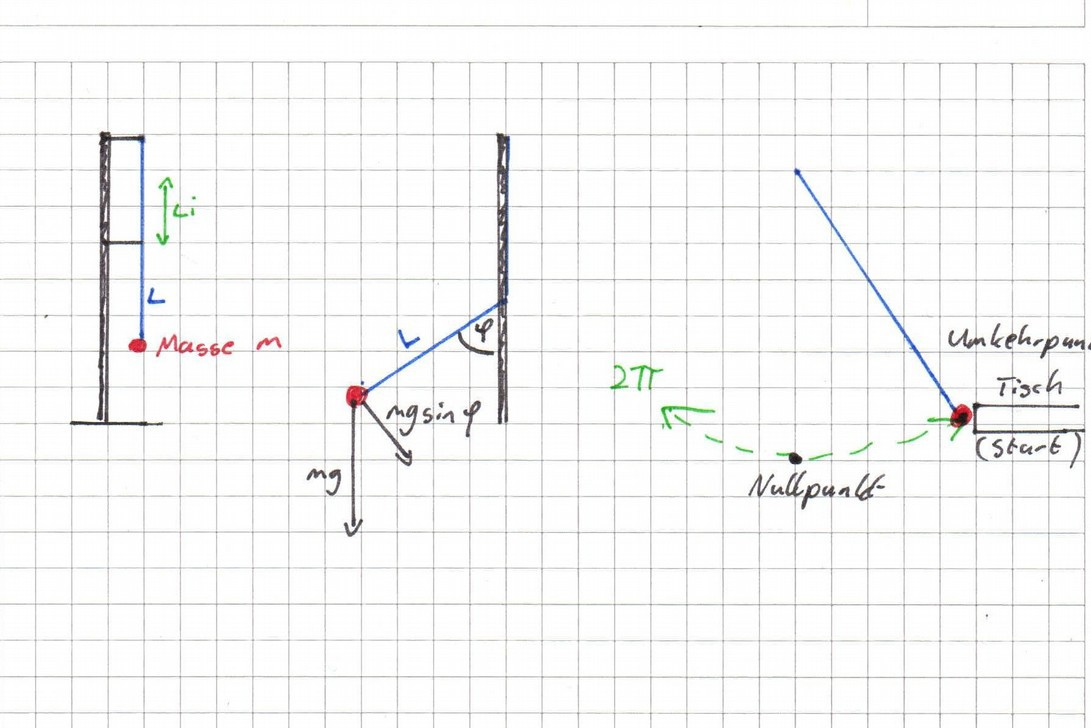
\includegraphics[scale=0.3]{Fadenpendel.png}
\caption{Fadenpendel}
\end{figure}
%Cassy die Schlampe
Da für die Bestimmung der Zeit/Schwingungsrelation bei einem Fadenpendel zwei Messpunkte (Messung bei Nulldurchgang bzw. am Wendepunkt) sowie Messdauer (eine gegenüber mehreren Schwingungen) möglich sind, werden zunächst die Standardabweichung der verschiedenen Methoden bestimmt und verglichen. Zunächst wird jeweils eine Messreihe für den Nullpunktdurchgang sowie den Umkehrpunkt mit einer Schwingungsdauer n = 10 bei 25 Wiederholungen aufgesetzt. Anschließend wird eine weitere Messreihe mit dem Nulldurchgang als Messpunkt und einer Schwingungsdauer $n=1$ durchgeführt. Mit der so bestätigten Messmethode und bestimmten Fehlergrößen kann nun im zweiten Teil die Erdbeschleunigung g errechnet werden. Hierfür wird eine dritte Messreihe mit sich von Messung  zu Messung um jeweils 4 cm ändernder Pendellänge (10 Schwingungen, Messung im Nullpunktdurchgang) durchgeführt. Für die Auswertung ist $T_{i2}$ gegen $L_i$ aufzutragen und die Geradensteigung zu berechnen. Durch die in den theoretischen Grundlagen etablierte Funktion $g = \frac{4\pi^2}{m}$ wird schließlich die Erdbeschleunigung bestimmt und mit dem Literaturwert verglichen.

\newpage
\textbf{Ergebnisse und Auswertung}\\Die Standardabweichung der drei verschiedenen Messungen variieren stark.
\begin{flushleft}
\begin{tabular}{l|ccc}
 & Nullpunktmessung & Umkehrpunktmessung & Nullpunktmessung\\
 & n=10 & n=10 & n=1\\
 \hline
Mittelwert & 1,736s & 1,695s & 1,493s\\
Standardabweichung & $\pm 0,008s$ & $\pm 0,015s$ & $\pm 0,126s$\\
Konfidenzintervall 95\% & $\pm 1,6\cdot10^{-3}$ & $\pm 3,3\cdot 10^{-3}$ & $ \pm 8 \cdot10^{-3}$\\
\end{tabular}
\end{flushleft}

Am größten ist die Standardabweichung bei der Bestimmung nur einer Periodendauer. Da hier die Messdauer $\frac{1}{n}\cdot \Sigma T \approx 1,5 s$ und die menschliche Reaktionszeit eine gewählte Messungenauigkeit von etwa $\pm 0,1s$ einbringt, beträgt die Standardabweichung beinahe 10 \% des Messwertes. Wird die Messung nun auf 10 Perioden heraufgesetzt verringert sich auch der Einfluss der Reaktionszeit als Fehler pro Schwingung deutlich, die Ergebnisse liegen folglich näher beieinander.Am Nullpunktdurchgang hingegen hat das Pendel seine maximale Geschwindigkeit erreicht, der für eine Messung infrage kommende Zeitpunkt ist deutlicher erkennbar, was sich in einer Halbierung der Standardabweichung niederschlägt. Für die Berechnung der Erdbeschleunigung $g$ wird schließlich $T_i^2$ gegen $L_i$ aufgetragen und die Steigung der Ausgleichsgeraden berechnet:\\
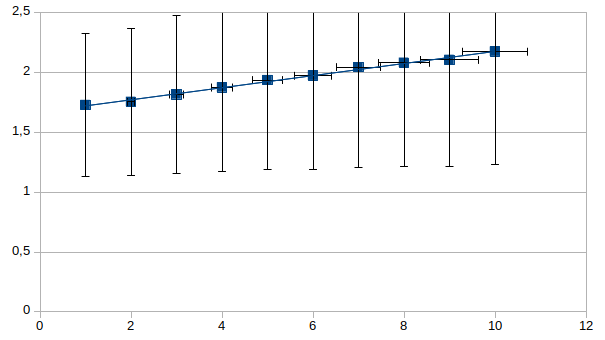
\includegraphics[scale=1]{Diagramm.png}\\
Es ergibt sich eine Steigung $m = 0,048\frac{s}{cm}$ Längenänderung. Eingesetzt in die, in den theoretischen Grundlagen, etablierte Formel $(\frac{4\pi}{m} = g)$
ergibt sich hieraus: $g = 833 \frac{cm}{s^2}\ (8,33\frac{m}{s^2})$. Dieser Wert weicht deutlich vom Literaturwert ($9,81\frac{m}{s^2}$) ab. Diese Differenz ist jedoch bei der Größe des menschlichen Einflussfaktors erwartbar. Die Reaktionszeit von etwa 0,1s sowie der wegen der Geschwindigkeit des Pendels nur mit großem Ermessensspielraum abschätzbare Zeitpunkt des Nullpunktdurchganges, haben das Potenzial den berechneten Wert stark zu verzerren. Schauen wir uns die Fehlerbereiche des Diagramms an, so sehen wir, dass die Fehlerbereiche doch großgenug sind, als dass Mittelgerade mit der Steigung von $9,81\frac{m}{s^2}$ durchaus möglich ist. Somit liegt der Erwartungswert des Experminetes innerhalb des Fehlerbereiches.

\end{document}